% online/offline; with/without reconstruction
% general, focus on backbone, no task-specific or model-specific design-->comparable performance is OK
% extend SV model to online perception, with only simple prediction fusion
% If possible, compare FPS and parameters

In this section, we first describe our datasets and implementation details. Then we compare our method with state-of-the-art methods on both room-level and online benchmarks to comprehensively analyze the advantage of memory-based adapters. Finally we conduct ablation studies to validate the effectiveness of our design.

\subsection{Benchmarks and Implementation Details}\label{impd}
We evaluate our method on two datasets: ScanNet~\cite{dai2017scannet} and SceneNN~\cite{hua2016scenenn}. ScanNet contains 1513 scanned scene sequences, out of which we use 1201 sequences for training and the rest 312 for testing. SceneNN is a smaller dataset which contains 50 high-quality scanned scene sequences with semantic label. After careful filtering, we select 12 clean sequences for testing. We train all models on ScanNet and evaluate them on ScanNet or SceneNN.

\textbf{Benchmarks:} We first compare different methods on room-level benchmarks, i.e., the performance on the reconstructed complete scenes. 
For semantic segmentation, we compare different methods on ScanNet and SceneNN. Since online methods may not perform 3D reconstruction, we map their predictions on point clouds concatenated from posed RGB-D images to the reconstructed point clouds with nearest neighbor interpolation. For object detection and instance segmentation, the metric is computed on each object rather than the whole point clouds. Therefore we use reconstructed point clouds and RGB-D videos as the inputs for offline and online methods respectively, and calculate metrics based on their respective inputs.

We also follow AnyView~\cite{wu2023anyview} to organize an online benchmark on ScanNet for more comprehensive evaluation. We divide the RGB-D video of each room into several non-overlapping sequences and regard each sequence as an independent scene, where the number or the length of each sequence can be set to different values. In this way, we can measure the generalization ability of different methods when the input scenes are incomplete and of variable scales, which is a more practical setting. In our experiments, we divide each room into 1/5/10 sequences or sequences with fixed length 5/10/15, resulting in 6 metrics.


\textbf{Implementation details:} To train $\mathcal{M}_{SV}$, we first train a 2D perception model $\mathcal{M}_{I}$ following Pri3D~\cite{hou2021pri3d}. We use UNet~\cite{ronneberger2015u} for semantic segmentation and Faster-RCNN~\cite{ren2016faster} (only ResNet~\cite{he2016deep} and FPN~\cite{lin2017fpn} backbones are needed) for object detection and instance segmentation. Then we fix the image backbone and train $\mathcal{M}_{SV}$ on ScanNet-25k~\cite{dai2017scannet}, which is a single-view RGB-D dataset. For online perception, we zero-initialize the memory-based adapters and insert them into $\mathcal{M}_{SV}$. Then we train the new model on RGB-D videos from ScanNet. To reduce memory footprint, we randomly sample 8 adjacent RGB-D frames for each scene at every iteration.
We insert our memory-based adapters between the backbone and neck. For backbones which output multi-level features, we insert different adapters to different levels. In terms of hyperparameters, we set $l=50$, $s=2.5$, $\tau=8$ and $\delta=0.03$. We simply use the same optimizer configurations to train the models as in their original paper (designed for offline training).

For prediction fusion, we adopt different strategies for different tasks. 
\emph{Semantic segmentation}: The predictions for each frame are concatenated, which has the same point number with $S_t$. We use 2$cm$ voxelization to unify the predictions for points inside the same voxel grid by channel-wise maxpooling. 
\emph{Object detection}: The predicted bounding boxes for each frame are merged by 3D NMS. When two boxes of different time are colliding during NMS, we add $\delta$ to the classification scores of box in the newer frame. This is because our method ensures the backbone extracts more complete geometric features for the newer frame.
\emph{Instance segmentation}: Instance segmentation can be divided into transformer-based~\cite{schult2022mask3d}, grouping-based~\cite{jiang2020pointgroup,vu2022softgroup} and detection-based~\cite{hou20193d,yi2019gspn,kolodiazhnyi2023top}. As the first two kinds require a specially designed mask fusion strategy~\cite{liu2022ins} for online perception, we opt for the detection-based manner, where we can first conduct online 3D object detection and then utlize the boxes to crop and segment the point cloud features stored in the memory.


\subsection{Comparison with State-of-the-art}
We compare our method with the top-performance offline and online 3D perception models. Offline models refer to $\mathcal{M}_{Rec}$ described in Section \ref{def}, which is trained on reconstructed point clouds. Models with suffix "-SV" refer to $\mathcal{M}_{SV}$ that is trained on single-view RGB-D images.

\begin{table}[t]
    \setlength{\tabcolsep}{4pt}
    \centering
    \caption{3D semantic segmentation results on ScanNet and SceneNN datasets. For online methods, we map the predictions on point clouds concatenated from posed RGB-D images to the reconstructed point clouds to compare with offline method.}\label{tab1}
    \begin{tabular}{lc|cc|cc}  
        \toprule
        \multirow{2}{*}{Method} & \multirow{2}{*}{Type} & \multicolumn{2}{c|}{ScanNet} & \multicolumn{2}{c}{SceneNN} \\
        & & mIoU & mAcc & mIoU & mAcc \\
        \midrule
        MkNet~\cite{choy20194d} & Offline &71.6 &80.4 &-- &-- \\
        \midrule
        Fs-A~\cite{zhang2020fusion} & Online &63.5 &73.7 &51.1 &62.4 \\
        \rowcolor{mygray} MkNet-SV & Online &68.8 &77.7 &48.4 &61.2 \\
        \rowcolor{mygray} MkNet-SV+Ours & Online &\textbf{72.7} &\textbf{84.1} &\textbf{56.7} &\textbf{70.1} \\
        \bottomrule
    \end{tabular}
\end{table}

\begin{table}[t]
    \setlength{\tabcolsep}{4pt}
    \centering
    \small
    \caption{3D object detection and instance segmentation results on ScanNet dataset. Offline and online methods are separated by horizontal line. $^\dag$ means INS-Conv requires an additional 3D reconstruction algorithm to acquire high-quality point clouds or meshes.}\label{tab2}
    \begin{tabular}{c|cc|c|cc}  
        \toprule
        \multicolumn{3}{c|}{Detection} & \multicolumn{3}{c}{Insseg} \\
        \midrule
        \multirow{2}{*}{Method} & \multicolumn{2}{c|}{mAP} & \multirow{2}{*}{Method} & \multicolumn{2}{c}{mAP} \\
        & @25 & @50 & & @25 & @50 \\
        \midrule
        FCAF3D~\cite{rukhovich2022fcaf3d} &70.7 &56.0 &SoftGroup~\cite{vu2022softgroup} &78.9 &67.6 \\
        CAGroup3D~\cite{wang2022cagroup3d} &74.5 &60.3 &TD3D~\cite{kolodiazhnyi2023top} &81.3 &71.1 \\
        \midrule
        AnyView~\cite{wu2023anyview} &60.4 &36.0 &INS-Conv$^\dag$~\cite{liu2022ins} &-- &57.4 \\
        \rowcolor{mygray} FCAF3D-SV &41.9 &20.6 &TD3D-SV & 53.7 &36.8 \\
        \rowcolor{mygray} FCAF3D-SV+Ours &\textbf{70.5} &\textbf{49.9} &TD3D-SV+Ours & \textbf{71.3} & \textbf{60.5} \\
        \bottomrule
    \end{tabular}
\end{table}

\begin{table*}[]
	\centering
	\setlength{\abovedisplayskip}{0pt}
	\setlength{\belowdisplayskip}{0pt}
    \small
	\caption{The performance of different 3D scene perception methods on ScanNet online benchmark. We report mIoU / mAcc, mAP@25 / mAP@50 and mAP@25 / mAP@50 for semantic segmentation, object detection and instance segmentation respectively.}\label{tab3}
	\begin{tabular}{c|l|p{1.5cm}<{\centering}|p{1.5cm}<{\centering}|p{1.5cm}<{\centering}|p{1.5cm}<{\centering}|p{1.5cm}<{\centering}|p{1.5cm}<{\centering}|p{1.5cm}<{\centering}}
		\toprule
		 & \multirow{2}{*}{Method} & \multirow{2}{*}{Type} & \multicolumn{3}{c|}{Number of Sequence} & \multicolumn{3}{c}{Length of Sequence} \\
         & & &\ 1\ &5\ &10 &5\ &10 &15 \\
		\midrule
        \multirow{4}{*}{\rotatebox[origin=c]{90}{Semseg}} &MkNet & Offline &63.7 / 73.5 &62.7 / 72.8 &58.9 / 69.4 &59.3 / 69.8 &63.0 / 73.0 &63.5 / 73.7 \\
        &Fs-A & Online &62.0 / 72.8 &60.6 / 71.7 &60.0 / 71.3 &60.1 / 71.3 &60.7 / 71.8 &61.0 / 72.0  \\
        &MkNet-SV & Online &63.3 / 74.3 &63.3 / 74.3 &63.3 / 74.3 &63.3 / 74.3 &63.3 / 74.3 &63.3 / 74.3  \\
        &MkNet-SV+Ours & Online &\textbf{69.1} / \textbf{82.2} &\textbf{66.8} / \textbf{80.0} &\textbf{65.9} / \textbf{79.2} &\textbf{65.9} / \textbf{79.3} &\textbf{66.8} / \textbf{80.1} &\textbf{67.1} / \textbf{80.4}  \\
		\midrule
        \multirow{4}{*}{\rotatebox[origin=c]{90}{Detection}} &FCAF3D & Offline &57.0 / 40.6 &41.1 / 25.2 &34.6 / 19.3 &28.4 / 15.2 &33.9 / 19.4 &37.7 / 22.8 \\
        &AnyView & Online &60.4 / 36.0 &48.8 / 25.3 &43.1 / 20.5 &36.6 / 16.5 &42.0 / 20.7 &45.6 / 23.8  \\
        &FCAF3D-SV & Online &41.9 / 20.6 &29.8 / 13.3 &27.0 / 11.5 &24.4 / 10.1 &26.2 / 11.0 &27.6 / 12.1 \\
        &FCAF3D-SV+Ours & Online &\textbf{70.5} / \textbf{49.9} &\textbf{58.7} / \textbf{37.7} &\textbf{56.2} / \textbf{34.3} &\textbf{53.1} / \textbf{31.2} &\textbf{54.9} / \textbf{33.8} &\textbf{56.1} / \textbf{35.6}  \\
        \midrule
        \multirow{3}{*}{\rotatebox[origin=c]{90}{Insseg}} &TD3D & Offline & 64.0 / 50.8 &61.6 / 49.7 &59.4 / 48.4 &59.0 / 47.9 &61.4 / 49.8 &61.7 / 49.8 \\
        &TD3D-SV & Online &53.7 / 36.8 &54.2 / 41.6 &57.0 / 46.3 &56.4 / 45.5 &53.9 / 40.9 &52.6 / 39.5 \\
        &TD3D-SV+Ours & Online &\textbf{71.3} / \textbf{60.5} &\textbf{64.7} / \textbf{55.2} &\textbf{64.2} / \textbf{55.0} &\textbf{64.0} / \textbf{54.7} &\textbf{64.6} / \textbf{55.1} &\textbf{63.9} / \textbf{54.3} \\
		\bottomrule
	   \end{tabular}
\end{table*}

\textbf{Room-level benchmarks:} By default, offline methods take in reconstructed point clouds and online methods take in posed RGB-D videos without 3D reconstruction. Special case is denoted by $^\dag$.
Note that there is a challenge in online methods when compare to offline alternatives, as offline methods directly process the complete and clean 3D geometry of rooms while online methods deal with partial and noisy frames. According to Table \ref{tab1} and Table \ref{tab2}, by simply inserting the memory-based adapters into $\mathcal{M}_{SV}$, we significantly boost their accuracy on complete scenes and achieve better performance compared with state-of-the-art online 3D scene perception models specially designed for each task. We observe the improvement upon $\mathcal{M}_{SV}$ is especially significant on 3D object detection and instance segmentation tasks. This is because these tasks require complete predictions for each object, while it is usually very hard to infer the whole geometry of large objects with a single RGB-D frame.
We also notice our method even outperforms offline methods on semantic segmentation task. Since this task requires more detailed perception of local geometry rather than the global context, our method can predict finer segmentation with only partial and noisy inputs.

\textbf{Online benchmark:} In this benchmark, the inputs to all methods are the posed RGB-D sequences. We concatenate the point clouds from each RGB-D frame of a sequence into a whole for offline methods. As the code of INS-Conv is not accessible, we do not compare with it on this benchmark. According to Table \ref{tab3}, offline methods show bad generalization ability on partial and noisy scenes, especially when the input sequence is short. Note that offline methods take in the whole observed scene $S_t$ at each time. When processing $S_{t+1}$, the features extracted for $S_t$ is wasted. On the contrary, online methods process a single frame $x_t$ at each time and fuse the per-frame predictions, which is much more efficient and practical in real-time robotic tasks. Equipped with our memory-based adapters, $\mathcal{M}_{SV}$ achieves the best performance compared with other offline and online methods on all tasks and experimental settings. We observe the longer the input sequence, the larger the improvement upon $\mathcal{M}_{SV}$, which validates our modules can effectively aggregate long-term temporal information.

\begin{table}[]
    \centering
    \setlength\tabcolsep{14pt}
    \caption{Ablation study on point cloud and image modules. We report semantic segmentation results on ScanNet. The performance of image module is based on point cloud module.}\label{tab45}
    \footnotesize
    \begin{tabular}{l|p{0.5cm}<{\centering}p{0.5cm}<{\centering}}
        \toprule
        Method & mIoU & mAcc \\
        \midrule
        Remove residual connection &64.6 &77.9 \\
        Random initialization &66.2 &78.6 \\
        Remove voxel maxpooling &64.8 &76.1 \\
        Set scaling factor $s=1$ &65.3 &78.4 \\
        Set scaling factor $s=5$ &66.8 &79.3 \\
        Insert after neck &66.0 &78.8 \\
        \textbf{The final point cloud module} &\textbf{66.9} &\textbf{79.3} \\
        \midrule
        Remove residual connection &67.1 &79.8 \\
        Random initialization &68.7 & 81.7 \\
        Set shift ratio $\tau=4$ &68.9 &82.1 \\
        Set shift ratio $\tau=16$ &68.7 &81.9 \\
        Remove 3D to 2D adapter &68.0 &80.8 \\
        Insert after neck &68.4 &81.6 \\
        \textbf{The final image module} &\textbf{69.1} &\textbf{82.2} \\
        \bottomrule
    \end{tabular}
\end{table}

\begin{table}[]
    \centering
    \setlength\tabcolsep{8pt}
    \caption{Effects of our memory-based adapters when both image and point cloud backbones are fixed during finetuning.}\label{tab6}
    \footnotesize
    \begin{tabular}{c|c|c|c}
        \toprule
         & MkNet & FCAF3D & TD3D \\
        \midrule
        Fix I &69.1 / 82.2 &70.5 / 49.9 &71.3 / 60.5 \\
        Fix P \& I &67.3 / 79.9 &66.4 / 47.1 &69.1 / 58.2 \\
        \bottomrule
    \end{tabular}
\end{table}

We visualize the predictions of different methods in Figure \ref{vis}. 
It can be seen that our method is more accurate than $\mathcal{M}_{SV}$ due to the temporal modeling ability, and more robust to number of frames than offline methods.
% SV methods fails to utilize temporal information and thus outputs noisy predictions.

\begin{figure*}[t]
    \centering
    \vspace{-1mm}
    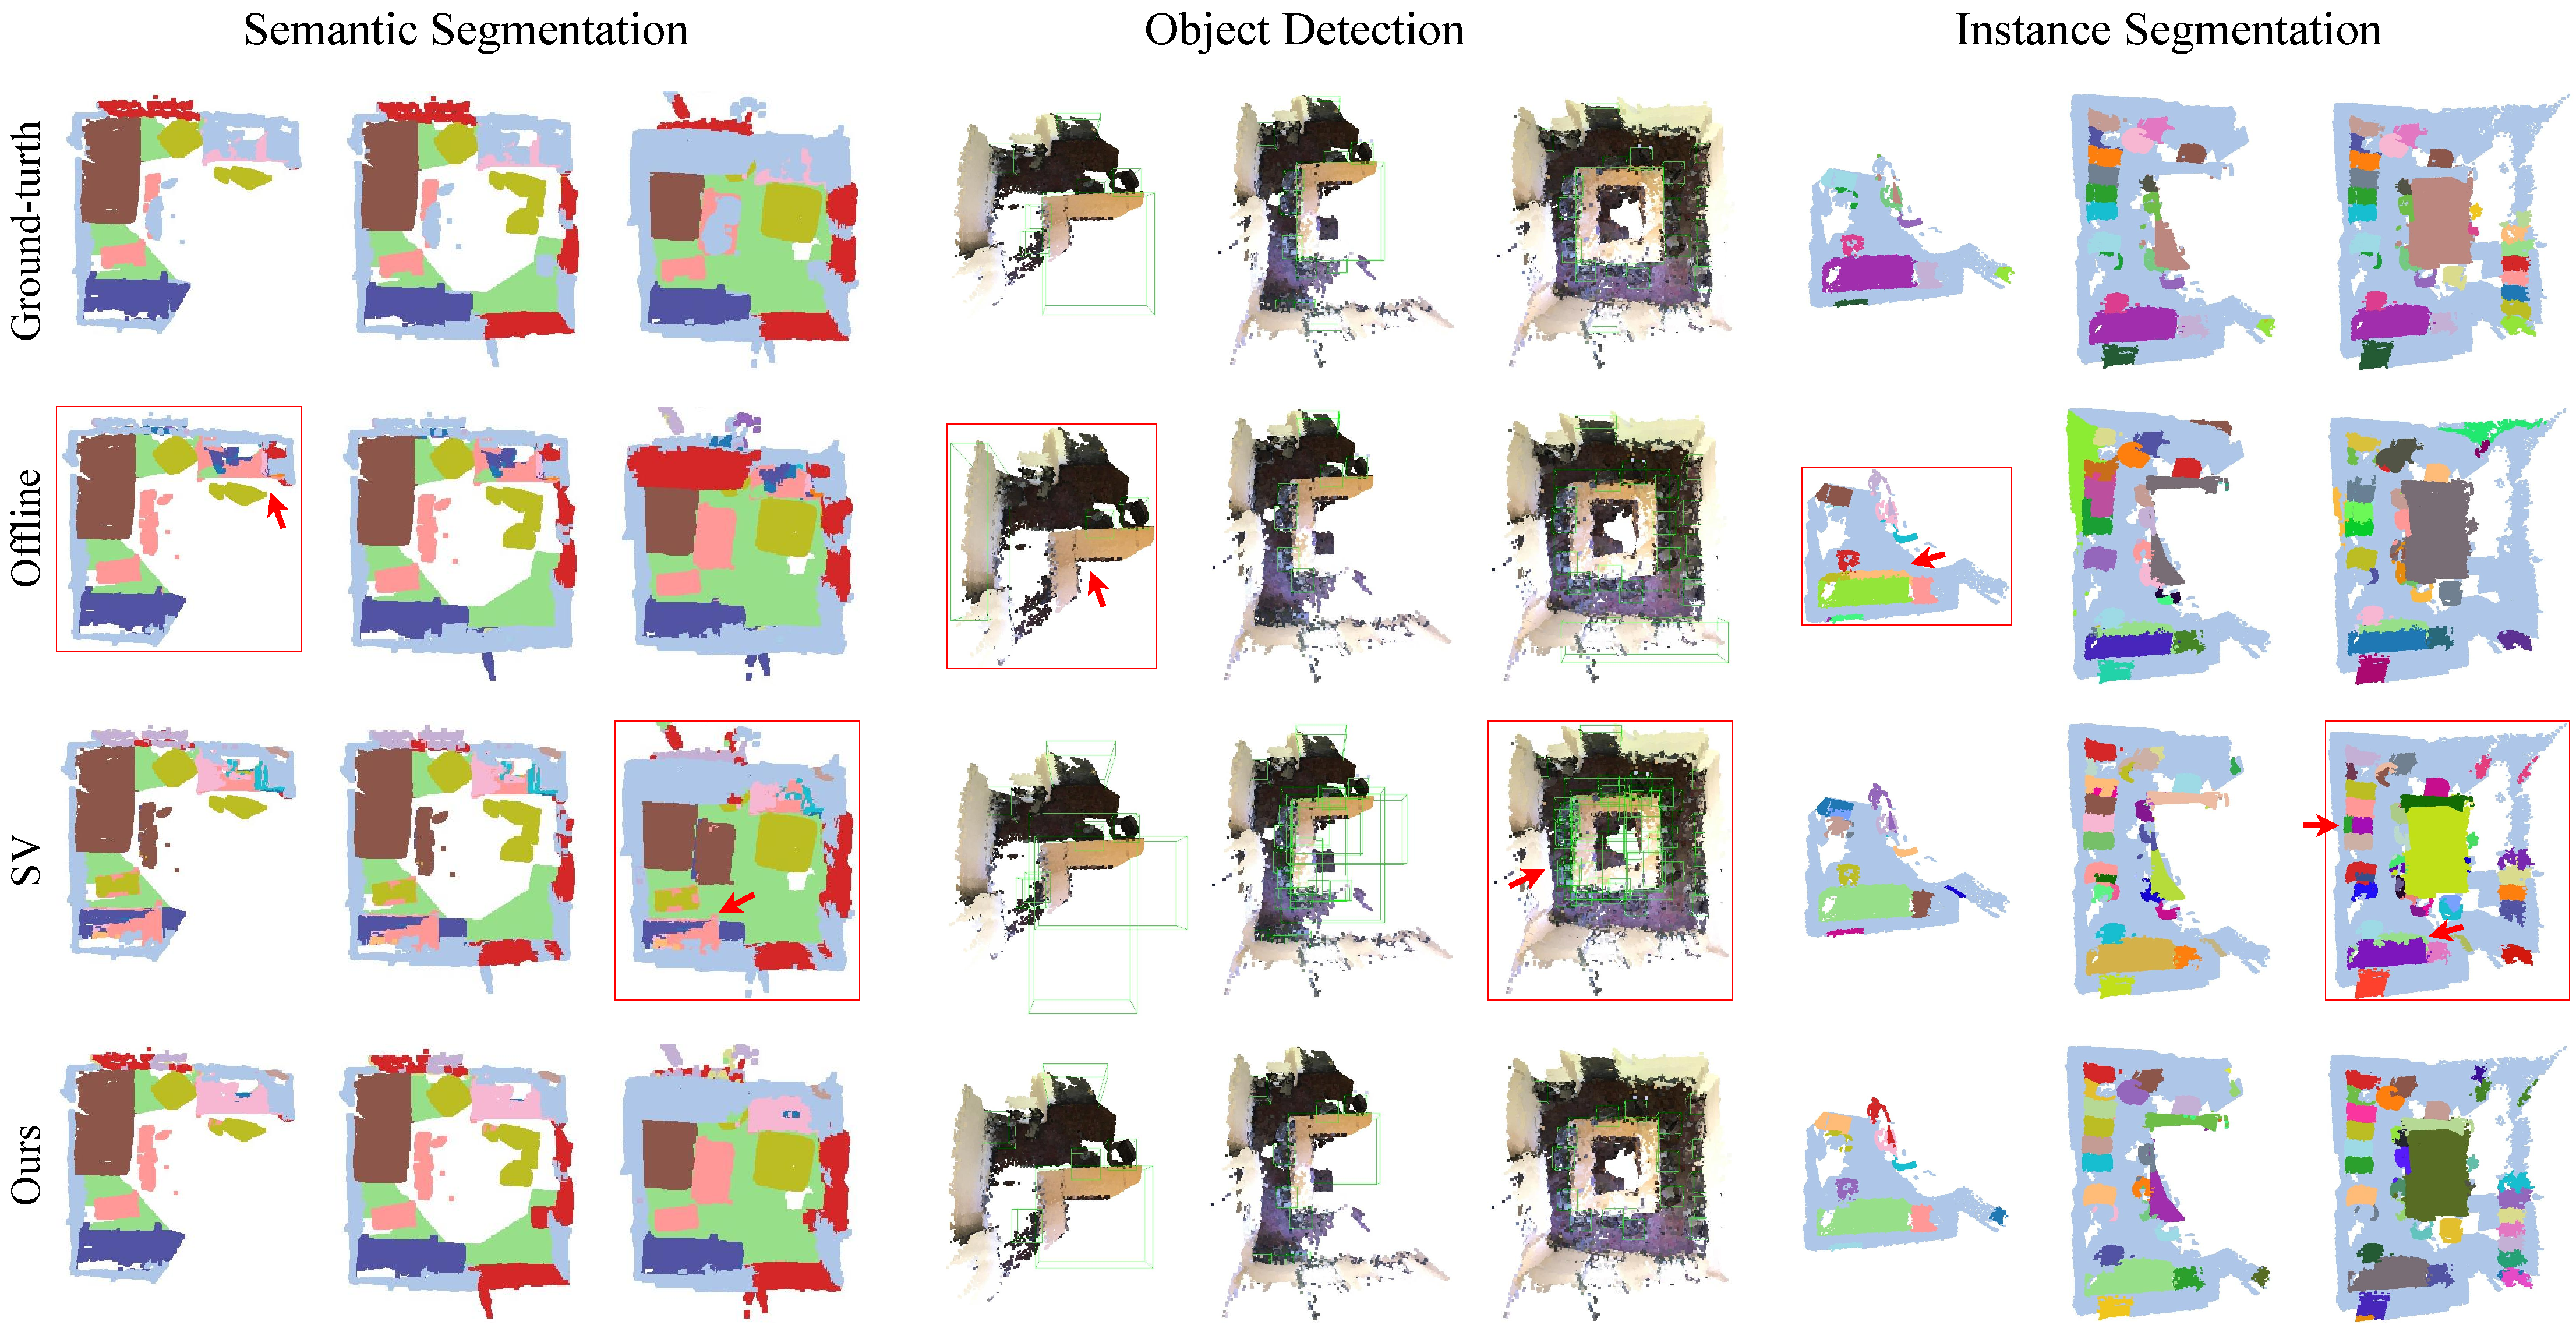
\includegraphics[width=\linewidth]{figures/exp.pdf}
    \caption{Visualization results on the online benchmark. Our predictions are accurate and robust to the number of frames. Note that some ground-truth masks are incomplete due to the noisy 2D annotations, in this case our predictions are more reasonable than the ground-truths.}
    \label{vis}
\end{figure*}

\subsection{Ablation Study}
We first ablate the design choices of two memory-based adapters on 3D semantic segmentation task on ScanNet. 
Besides, we further show the performance of our method when both image and point cloud backbones are fixed during finetuning the adapters. 
% For all methods, we evaluate them on the online benchmark (Number of Sequence is 1).

% \begin{table}[]
%     \centering
%     \setlength\tabcolsep{10pt}
%     \caption{Comparison of different design choices of the image module. We report semantic segmentation results on ScanNet based on the point cloud module.}\label{tab5}
%     \begin{tabular}{l|p{0.5cm}<{\centering}p{0.5cm}<{\centering}}
%         \toprule
%         Method & mIoU & mAcc \\
%         \midrule
%         Remove residual connection &67.1 &79.8 \\
%         Random initialization &68.7 & 81.7 \\
%         Set shift ratio $\tau=4$ &68.9 &82.1 \\
%         Set shift ratio $\tau=16$ &68.7 &81.9 \\
%         Remove 3D to 2D adapter &68.0 &80.8 \\
%         Insert after neck &68.4 &81.6 \\
%         \textbf{The final image module} &\textbf{69.1} &\textbf{82.2} \\
%         \bottomrule
%     \end{tabular}
% \end{table}

% \begin{table}[]
%     \centering
%     \setlength\tabcolsep{8pt}
%     \caption{Effects of our memory-based adapters when both image and point cloud backbones are fixed during finetuning.}
%     \begin{tabular}{l|cc|c}
%         \toprule
%         \multirow{2}{*}{Method} & \multicolumn{2}{c|}{Fixed Backbone} & \multirow{2}{*}{Performance} \\
%          & Image & Point & \\
%         \midrule
%         MkNet-SV+Ours &\checkmark & & \\
%         MkNet-SV+Ours &\checkmark &\checkmark & \\
%         \midrule
%         FCAF3D-SV+Ours &\checkmark & & \\
%         FCAF3D-SV+Ours &\checkmark &\checkmark & \\
%         \midrule
%         TD3D-SV+Ours &\checkmark & & \\
%         TD3D-SV+Ours &\checkmark &\checkmark & \\
%         \bottomrule
%     \end{tabular}
% \end{table}

\textbf{Point cloud and image modules:} Table \ref{tab45} validates the effectiveness of our designs. We observe removing voxel maxpooling significantly degrades the performance, which shows the importance of updating memory. With the increase of $s$, the performance first improves and then keeps steady or even slightly declines, which indicates the neighbor context information is important for temporal learning, but too large neighbor voxel set brings much redundant features. 
Large $s$ will also increase the computation overhead, so we choose $s=2.5$ to achieve the best accuracy-computation tradeoff.
% Table \ref{tab45} validates the effectiveness of the memory-based adapter for image features as well as the 3D-to-2D adapter. 
We observe the influence of $\tau$ is similar with $s$ and thus choosing a proper value is important for both high accuracy and less memory storage. From these experiments, we also validate the effectiveness of the 'adapter paradigm', which includes residual connection, zero-initialization and inserting after backbone.


\textbf{Fixed backbones:} When finetuning our adapters, we fix the image backbone and finetune other parameters. We further study the effects of our method when both image and point cloud backbones are fixed. As shown in Table \ref{tab6}, even with both image and point cloud backbones fixed, our method still achieves state-of-the-art performance on all three online tasks. In this way, we can further reduce the memory footprint and training time, which provides the users with more efficiency-accuracy tradeoff.